\documentclass[a4paper,12pt]{article}
\usepackage[ukrainian,english]{babel}
\usepackage{ucs}
\usepackage[utf8]{inputenc}
\usepackage[T2A]{fontenc}
\usepackage{graphicx}
\usepackage{wrapfig}
\begin{document}
\title{Моделі сучасної фізики}
\maketitle
\date{ }
<математичні моделі взаємодії матеріальних об'єктів і будови матерії>

\newpage
\tableofcontents
\newpage
\section{Вступ}
\textbf{В.1. Сучасна модель будови Всесвіту}

\textbf{макросвіт}(елементарні частки, ядра, атоми)$\rightarrow$\textbf{мікросвіт}(окремі зікрки і системи планет)$\rightarrow$\textbf{мегасвіт}(скупчення зірок, галактики, скупчення галактик, Всесвіт в цілому)

Наука, що вивчає походження і будову Всесвіту має назву "Космологія".
Наша галактика: Галактика, або "Чумацький шлях".
\\"the Big Bang" - великий "вибух": $\Delta t\approx 13\cdot 10^9 \textrm{ років}, \approx 10^{26}\textrm{ м}.$
\\Розширення Всесвіту, з. Хаббла: $V=Hr$; галактики - свого роду "атоми" Всесвіту, розбігання галактик.
Будь-яка галактіка - гравітаційно зв'язана система зірок, занурених у газі "темну матерію", природа якої, поки що, невідома. Форми галактик: неправильні, сферичні, елісоїдні, спіральні, кульові.\\
Наша галактика:

\begin{wrapfigure}{R}{0.5\textwidth}
\centering
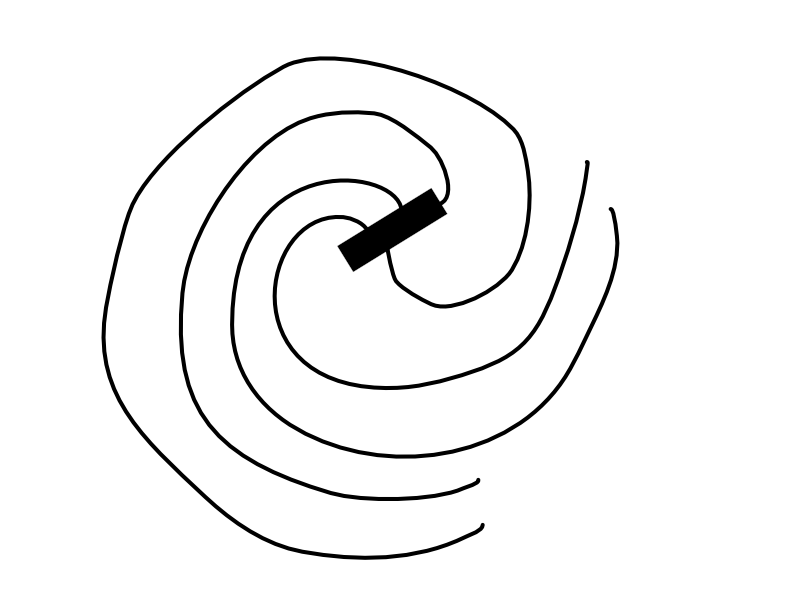
\includegraphics[width=0.4\textwidth]{galaxy}
\end{wrapfigure}
п'ять рукавів:\begin{enumerate}
	\item Лебедя
\item Оріона
\item Персея
\item Стрільця
\item Центаври
\end{enumerate}


\end{document}

